\documentclass{beamer}
\usepackage[utf8]{inputenc}
\usepackage{graphicx, epsfig}
\usepackage{amsmath,mathrsfs,amsfonts,amssymb}
\usepackage{floatflt}
\usepackage{epic,ecltree}
\usepackage{mathtext}
\usepackage{fancybox}
\usepackage{fancyhdr}
\usepackage{multirow}
\usepackage{enumerate}
\usepackage{epstopdf}
\usepackage{multicol}
\usepackage{algorithm}
\usepackage[noend]{algorithmic}
\usepackage{tikz}
\usepackage{blindtext}
\usepackage{multido}
\usetheme{default}%{Singapore}%{Warsaw}%{Warsaw}%{Darmstadt}
\usecolortheme{default}

\setbeamerfont{title}{size=\Huge}
\setbeamertemplate{footline}[frame number]{}

\setbeamertemplate{section in toc}[sections numbered]

\makeatletter
\newcommand\HUGE{\@setfontsize\Huge{35}{40}}
\makeatother    

\setbeamerfont{title}{size=\HUGE}
\beamertemplatenavigationsymbolsempty

\usetikzlibrary{arrows,shapes,positioning,shadows,trees}

\newcommand\myfootnote[1]{%
  \vspace{-0.5cm}%
  \tikz[remember picture,overlay]
  \draw (current page.south west) +(1in + \oddsidemargin,0.5em)
  node[anchor=south west,inner sep=0pt]{\parbox{\textwidth}{%
      \rlap{\rule{10em}{0.4pt}}\raggedright\scriptsize \textit{#1}}};}

\newcommand\myfootnotewithlink[2]{%
  \vspace{-0.5cm}%
  \tikz[remember picture,overlay]
  \draw (current page.south west) +(1in + \oddsidemargin,0.5em)
  node[anchor=south west,inner sep=0pt]{\parbox{\textwidth}{%
      \rlap{\rule{10em}{0.4pt}}\raggedright\scriptsize\href{#1}{\textit{#2}}}};}

\AtBeginSection[]
      {
      	\begin{frame}{Outline}
      		\tableofcontents[currentsection]
      	\end{frame}
      }
      \AtBeginSubsection[]{
      	\begin{frame}{Outline}
      		\tableofcontents[currentsection,currentsubsection]
      	\end{frame}
}

\newcounter{noscounter} % Используется для nextonslide команды (обнуляется только на новом слайде)
\newcounter{pcounter} % Используется для pause команды (обнуляется после использования eqpause)
\newcounter{diffcounter} % Считает количество pause после формулы

\newcommand{\nextonslide}[1]{%
  \stepcounter{noscounter}% Прибавляем счетчик nextonslide
  \stepcounter{pcounter}% Прибавляем счетчик pause
  \stepcounter{diffcounter}% Прибавляем счетчик diffcounter
  \onslide<\value{noscounter}->{#1}% Отображаем аргумент в скобках на слайде с номером noscounter
}
\newcommand{\resetonslide}{%
    \setcounter{noscounter}{1}% Сбрасываем счетчик nextonslide
    \setcounter{pcounter}{1}% Сбрасываем счетчик pause
    \setcounter{diffcounter}{0}% Сбрасываем счетчик diffcounter
}

\newcommand{\eqpause}{%
  \multido{\i=1+1}{\value{pcounter}}{\pause}% Повторяем pcounter раз команду pause
  \stepcounter{noscounter}% Прибавляем счетчик nextonslide
  \setcounter{pcounter}{1}% Сбрасываем счетчик pause
}

\newcommand{\eqpausediff}{% Вспомогательная команда, запускается автоматически после формул
  \multido{\i=1+1}{\value{diffcounter}}{\pause}% Повторяем diffcounter раз команду pause
  \addtocounter{pcounter}{-\value{diffcounter}}% Вычитаем из pcounter количество сделанных pause
  \setcounter{diffcounter}{0}% Сбрасываем счетчик diffcounter
}

\newcommand\AtEndBoth[2]{% Применяем команду к multline и multline*
  \AtEndEnvironment{#1}{#2}%
  \AtEndEnvironment{#1*}{#2}%
}

\AtEndBoth{align}{\eqpausediff}
\AtEndBoth{equation}{\eqpausediff}
\AtEndBoth{multline}{\eqpausediff}

\addtobeamertemplate{frametitle}{\resetonslide}{}% На каждом слайде сбрасываем счетчики

% latin bold lower
\newcommand{\ba}{\mathbf{a}} 
\newcommand{\bc}{\mathbf{c}} 
\newcommand{\be}{\mathbf{e}} 
\newcommand{\bff}{\mathbf{f}} % \bf - for bold type
\newcommand{\bg}{\mathbf{g}} 
\newcommand{\bh}{\mathbf{h}} 
\newcommand{\bp}{\mathbf{p}} 
\newcommand{\bq}{\mathbf{q}} 
\newcommand{\bt}{\mathbf{t}} 
\newcommand{\bs}{\mathbf{s}} 
\newcommand{\bu}{\mathbf{u}} 
\newcommand{\bv}{\mathbf{v}} 
\newcommand{\bw}{\mathbf{w}} 
\newcommand{\bx}{\mathbf{x}} 
\newcommand{\by}{\mathbf{y}} 
\newcommand{\bz}{\mathbf{z}} 

% latin bold upper
\newcommand{\bA}{\mathbf{A}} 
\newcommand{\bB}{\mathbf{B}} 
\newcommand{\bC}{\mathbf{C}} 
\newcommand{\bG}{\mathbf{G}} 
\newcommand{\bI}{\mathbf{I}} 
\newcommand{\bJ}{\mathbf{J}} 
\newcommand{\bL}{\mathbf{L}} 
\newcommand{\bM}{\mathbf{M}} 
\newcommand{\bP}{\mathbf{P}}
\newcommand{\bQ}{\mathbf{Q}} 
\newcommand{\bR}{\mathbf{R}} 
\newcommand{\bT}{\mathbf{T}} 
\newcommand{\bU}{\mathbf{U}} 
\newcommand{\bV}{\mathbf{V}} 
\newcommand{\bW}{\mathbf{W}} 
\newcommand{\bX}{\mathbf{X}} 
\newcommand{\bY}{\mathbf{Y}} 
\newcommand{\bZ}{\mathbf{Z}} 

% latin cal upper
\newcommand{\cF}{\mathcal{F}} 
\newcommand{\cG}{\mathcal{G}} 
\newcommand{\cI}{\mathcal{I}} 
\newcommand{\cL}{\mathcal{L}} 
\newcommand{\cM}{\mathcal{M}} 
\newcommand{\cN}{\mathcal{N}} 
\newcommand{\cP}{\mathcal{P}} 
\newcommand{\cS}{\mathcal{S}} 
\newcommand{\cT}{\mathcal{T}} 
\newcommand{\cW}{\mathcal{W}} 
\newcommand{\cX}{\mathcal{X}} 
\newcommand{\cZ}{\mathcal{Z}} 

% latin bb upper
\newcommand{\bbE}{\mathbb{E}} 
\newcommand{\bbI}{\mathbb{I}} 
\newcommand{\bbP}{\mathbb{P}} 
\newcommand{\bbR}{\mathbb{R}} 

% greek bold lower
\newcommand{\bepsilon}{\boldsymbol{\epsilon}} 
\newcommand{\btheta}{\boldsymbol{\theta}} 
\newcommand{\blambda}{\boldsymbol{\lambda}} 
\newcommand{\bpi}{\boldsymbol{\pi}} 
\newcommand{\bmu}{\boldsymbol{\mu}} 
\newcommand{\bsigma}{\boldsymbol{\sigma}} 
\newcommand{\bphi}{\boldsymbol{\phi}} 

% greek bold upper
\newcommand{\bSigma}{\boldsymbol{\Sigma}} 

\DeclareMathOperator*{\argmin}{arg\,min}
\DeclareMathOperator*{\argmax}{arg\,max}
\newcommand{\createdgmtitle}[1]{\title[\hbox to 56mm{Deep Generative Models  \hfill\insertframenumber\,/\,\inserttotalframenumber}]
	{\vspace{1cm} \\ \textbf{Deep Generative Models} \\ {\Huge Lecture #1}}
	\author{Roman Isachenko}
	\institute{
		Moscow Institute of Physics and Technology \\
		Yandex School of Data Analysis
	}
	\date{2025, Autumn}
}
\createdgmtitle{10}

%--------------------------------------------------------------------------------
\begin{document}
%--------------------------------------------------------------------------------
\begin{frame}[noframenumbering,plain]
\titlepage
	\resetonslide	
\end{frame}
%=======
\begin{frame}{Recap of Previous Lecture}
	\myfootnotewithlink{https://arxiv.org/abs/2006.11239}{Ho J. Denoising Diffusion Probabilistic Models, 2020}

	\textbf{Forward Process}: Converts an arbitrary distribution $\pd(\bx)$ into the standard normal $\cN(0, \bI)$ by incrementally adding noise.
	\begin{align*}
		q(\bx_t | \bx_{t-1}) &= \cN(\sqrt{1 - \beta_t}\, \bx_{t-1}, \beta_t\, \bI); \\
		q(\bx_t | \bx_0) &= \cN(\sqrt{\bar{\alpha}_t}\, \bx_0, (1 - \bar{\alpha}_t)\, \bI).
	\end{align*}
	\textbf{Reverse Process}: This intractable distribution can be well-approximated by a Gaussian (with unknown parameters) when $\beta_t$ is sufficiently small.
	\[
		q(\bx_{t-1}|\bx_{t}) = \frac{q(\bx_{t}|\bx_{t-1}) q(\bx_{t-1})}{q(\bx_{t})} \approx \cN \left(\bmu_{\btheta, t}(\bx_t), \bsigma_{\btheta, t}^2(\bx_t)\right)
	\]
	\textbf{Conditioned Reverse Process}: This Gaussian, with known parameters, describes how to denoise a noisy image~$\bx_t$ when the final clean image~$\bx_0$ is known.
	\[
		q(\bx_{t-1}|\bx_{t}, {\color{olive}\bx_0}) = \cN(\tilde{\bmu}_t(\bx_t, \bx_0), \tilde{\beta}_t\, \bI)
	\]
\end{frame}
%=======
\begin{frame}{Recap of Previous Lecture}
	\myfootnotewithlink{https://ayandas.me/blog-tut/2021/12/04/diffusion-prob-models.html}{Das A. An introduction to Diffusion Probabilistic Models, blog post, 2021}
	\begin{itemize}
		\item $\bz = (\bx_1, \dots, \bx_T)$ represents the latent variables.
		\item Variational posterior distribution:
		\vspace{-0.2cm}
		\[
			q(\bz | \bx) = q(\bx_1, \dots, \bx_T | \bx_0) = \prod_{t = 1}^T q(\bx_t | \bx_{t - 1}).
		\]
		\vspace{-0.3cm}
		\item Generative model and prior:
		\vspace{-0.2cm}
		\[
			\pt(\bx | \bz) = \pt(\bx_0 | \bx_1); \quad 
			\pt(\bz) = \prod_{t=2}^T \pt(\bx_{t - 1} | \bx_t) \cdot p(\bx_T)
		\]
	\end{itemize}
	\vspace{-0.2cm}
	\begin{block}{ELBO}
		\vspace{-0.2cm}
		\[
			\log \pt(\bx) \geq \bbE_{q({\color{teal}\bz} | \bx)} \log \frac{\pt(\bx, {\color{teal}\bz})}{q({\color{teal}\bz} | \bx)} = \cL_{\bphi, \btheta}(\bx) \rightarrow \max_{q, \btheta}
		\]
		\vspace{-0.5cm}
		\begin{multline*}
			\cL_{\bphi, \btheta}(\bx) =  {\color{olive}\bbE_{q(\bx_1 | \bx_0)} \log \pt(\bx_0 | \bx_1)} - {\color{violet}\KL\bigl(q(\bx_T | \bx_0) \| p(\bx_T)\bigr)} - \\
			- \sum_{t=2}^T  \underbrace{ \bbE_{q(\bx_t | \bx_0)}\KL \bigl(q(\bx_{t-1} | \bx_t, \bx_0) \| \pt(\bx_{t-1} | \bx_t)\bigr)}_{\cL_t}
		\end{multline*}
	\end{block}
\end{frame}
%=======
\begin{frame}{Recap of Previous Lecture}
	\myfootnotewithlink{https://arxiv.org/abs/2006.11239}{Ho J. Denoising Diffusion Probabilistic Models, 2020}
	\begin{block}{ELBO of the Gaussian Diffusion Model}
		\vspace{-0.7cm}
		\begin{multline*}
			\cL_{\bphi, \btheta}(\bx) =  {\color{olive}\bbE_{q(\bx_1 | \bx_0)} \log \pt(\bx_0 | \bx_1)} - {\color{violet}\KL\bigl(q(\bx_T | \bx_0) \| p(\bx_T)\bigr)} - \\
			- \sum_{t=2}^T  \underbrace{ \bbE_{q(\bx_t | \bx_0)}\KL \bigl(q(\bx_{t-1} | \bx_t, \bx_0) \| \pt(\bx_{t-1} | \bx_t)\bigr)}_{\cL_t}
		\end{multline*}
		\vspace{-1.0cm}
	\end{block}
	\begin{align*}
		q(\bx_{t-1} | \bx_t, \bx_0) &= \cN(\tilde{\bmu}_t(\bx_t, \bx_0), \tilde{\beta}_t \bI), \\
		\pt(\bx_{t - 1} | \bx_t) &= \cN \bigl(\bmu_{\btheta, t}(\bx_t), {\color{violet}\bsigma_{\btheta, t}^2(\bx_t)}\bigr)
	\end{align*}
	It is assumed that ${\color{violet}\bsigma_{\btheta, t}^2(\bx_t) = \tilde{\beta}_t \bI}$.
	\[
		\cL_t = \bbE_{q(\bx_t | \bx_0)} \left[\frac{1}{2\tilde{\beta}_t} \bigl\| \tilde{\bmu}_t(\bx_t, \bx_0) - \bmu_{\btheta, t}(\bx_t) \bigr\|^2  \right]
	\]
\end{frame}
%=======
\begin{frame}{Recap of Previous Lecture}
	\myfootnotewithlink{https://arxiv.org/abs/2006.11239}{Ho J. Denoising Diffusion Probabilistic Models, 2020}
	\[
		\cL_t = \bbE_{\color{violet}q(\bx_t | \bx_0)} \left[ {\color{olive}\frac{1}{2\tilde{\beta}_t}} \bigl\| \tilde{\bmu}_t(\bx_t, \bx_0) - \bmu_{\btheta, t}(\bx_t) \bigr\|^2  \right]
	\]
	\vspace{-0.3cm}
	\begin{block}{Reparameterization}
		\vspace{-0.7cm}
		\begin{align*}
			\tilde{\bmu}_t(\bx_t, \bx_0) &= \frac{1}{\sqrt{\alpha_t}} \cdot \bx_t - \frac{1 - \alpha_t}{\sqrt{\alpha_t (1 - \bar{\alpha}_t)}} \cdot \bepsilon \\
			\bmu_{\btheta, t}(\bx_t) &= \frac{1}{\sqrt{\alpha_t}} \cdot \bx_t - \frac{1 - \alpha_t}{\sqrt{\alpha_t (1 - \bar{\alpha}_t)}} \cdot \bepsilon_{\btheta, t}({\color{teal}\bx_t})
		\end{align*}
		\vspace{-0.7cm}
	\end{block}
	\vspace{-0.2cm}
	\[
		\cL_t  =	 \bbE_{\color{violet}\bepsilon \sim \cN(0, \bI)} \left[ \frac{(1 - \alpha_t)^2}{2\tilde{\beta}_t \alpha_t (1 - \bar{\alpha}_t)} \Bigl\| \bepsilon - \bepsilon_{\btheta, t}\bigl( {\color{teal}\sqrt{\bar{\alpha}_t} \bx_0 + \sqrt{1 - \bar{\alpha}_t} \bepsilon}\bigr) \Bigr\|^2 \right]
	\]
	At each step in the reverse diffusion process, our goal is to predict the noise~$\bepsilon$ added by the forward process!
	\begin{block}{Simplified Objective}
		\vspace{-0.7cm}
		\[
			 \cL_{\text{simple}} = \bbE_{t \sim U\{2, T\}} \bbE_{\bepsilon \sim \cN(0, \bI)} \Bigl\| \bepsilon - \bepsilon_{\btheta, t}\bigl( \sqrt{\bar{\alpha}_t} \bx_0 + \sqrt{1 - \bar{\alpha}_t} \bepsilon\bigr) \Bigr\|^2 
		\]
	\end{block}
\end{frame}
%=======
\begin{frame}{Recap of Previous Lecture}
	\myfootnotewithlink{https://arxiv.org/abs/2006.11239}{Ho J. Denoising Diffusion Probabilistic Models, 2020}
	\begin{block}{Training DDPM}
		\begin{enumerate}
			\item Draw a sample $\bx_0 \sim \pd(\bx)$.
			\item Sample a timestep $t \sim U\{1, T\}$ and noise $\bepsilon \sim \cN(0, \bI)$.
			\item Obtain the noisy image: $\bx_t = \sqrt{\bar{\alpha}_t} \cdot \bx_0 + \sqrt{1 - \bar{\alpha}_t} \cdot \bepsilon$.
			\item Compute the loss: $ \cL_{\text{simple}} = \| \bepsilon - \bepsilon_{\btheta, t}(\bx_t) \|^2 $.
		\end{enumerate}
	\end{block}
	\begin{block}{Sampling with DDPM}
		\begin{enumerate}
			\item Sample $\bx_T \sim \cN(0, \bI)$.
			\item Compute the mean of $\pt(\bx_{t-1} | \bx_t) = \cN(\bmu_{\btheta, t}(\bx_t), \sigma_t^2 \cdot \bI)$:
			\[
				\bmu_{\btheta, t}(\bx_t) = \frac{1}{\sqrt{\alpha_t}} \cdot \bx_t - \frac{1 - \alpha_t}{\sqrt{\alpha_t (1 - \bar{\alpha}_t)}} \cdot \bepsilon_{\btheta, t}(\bx_t)
			\]
			\vspace{-0.3cm}
			\item Generate a denoised image: $\bx_{t - 1} = \bmu_{\btheta, t}(\bx_t) +  \sigma_t \cdot \bepsilon$, where $\bepsilon \sim \cN(0, \bI)$.
		\end{enumerate}
	\end{block}
\end{frame}
%=======
\begin{frame}{Outline}
	\tableofcontents
\end{frame}
%=======
\section{DDPM as a Score-Based Generative Model}
%=======
\begin{frame}{Denoising Diffusion as a Score-Based Generative Model}
	\myfootnotewithlink{https://arxiv.org/abs/2006.11239}{Ho J. Denoising Diffusion Probabilistic Models, 2020}
	\begin{block}{DDPM Objective}
		\vspace{-0.7cm}
		\begin{align*}
			\cL_t &= \bbE_{\bepsilon \sim \cN(0, \bI)} \left[ \frac{(1 - \alpha_t)^2}{2\tilde{\beta}_t \alpha_t  (1 - \bar{\alpha}_t)}  \left\|  \bepsilon_{\btheta, t} (\bx_t) - \bepsilon\right\|_2^2  \right] \\
			\nextonslide{
			& = \bbE_{\bepsilon \sim \cN(0, \bI)} \left[ \frac{(1 - \alpha_t)^2}{2\tilde{\beta}_t \alpha_t }  \Bigl\| {\color{violet} \frac{\bepsilon_{\btheta, t}  (\bx_t) }{\sqrt{1 - \bar{\alpha}_t}}} - {\color{teal}\frac{\bepsilon}{\sqrt{1 - \bar{\alpha}_t}}}\Bigr\|_2^2  \right]
			}
		\end{align*}
		\vspace{-0.7cm}
	\end{block}
	\eqpause
	\vspace{-0.5cm}
	\begin{align*}
		q(\bx_t | \bx_0) &= \cN(\sqrt{\bar{\alpha}_t} \cdot \bx_0, (1 - \bar{\alpha}_t) \cdot \bI) \\
		\nextonslide{\nabla_{\bx_t} \log q(\bx_t | \bx_0) &= - \frac{\bx_t - \sqrt{\bar{\alpha}_t} \cdot \bx_0}{1 - \bar{\alpha}_t} = {\color{teal}-  \frac{\bepsilon}{\sqrt{1 - \bar{\alpha}_t}}}.}
	\end{align*}
	\eqpause
	We can reparameterize the model as: 
		\vspace{-0.2cm}
		\[
			\bs_{\btheta, t}(\bx_t) = {\color{violet}- \frac{\bepsilon_{\btheta, t}(\bx_t)}{\sqrt{1 - \bar{\alpha}_t}}} = \nabla_{\bx_t} \log \pt(\bx_t).
		\]
		\vspace{-0.3cm}
		\eqpause
		\[
			\cL_t = \bbE_{q(\bx_t | \bx_0)} \left[ \frac{(1 - \alpha_t)^2}{2\tilde{\beta}_t \alpha_t}  \Bigl\|  \bs_{\btheta, t} (\bx_t) - \nabla_{\bx_t} \log q(\bx_t | \bx_0) \Bigr\|_2^2  \right]
		\]
\end{frame}
%=======
\begin{frame}{DDPM vs NCSN: Objectives}
	\myfootnotewithlink{https://arxiv.org/abs/2006.11239}{Ho J. Denoising Diffusion Probabilistic Models, 2020}
	\begin{block}{DDPM Objective}
		\vspace{-0.5cm}
		\[
			\bbE_{\pd(\bx_0)} \bbE_{t \sim U\{1, T\}}\bbE_{q(\bx_t | \bx_0)} \left[ {\color{olive}\frac{(1 - \alpha_t)^2}{2\tilde{\beta}_t \alpha_t}} \Bigl\|  \bs_{\btheta, t} (\bx_t) - \nabla_{\bx_t} \log q(\bx_t | \bx_0) \Bigr\|_2^2  \right]
		\]
		\[
			\bx_t = \sqrt{\bar{\alpha}_t} \cdot \bx_0 + \sqrt{1 - \bar{\alpha}_t} \cdot \bepsilon
		\]
		\eqpause
		In practice, {\color{olive}this coefficient} is often omitted.
	\end{block}
	\eqpause
	\begin{block}{NCSN Objective}
		\vspace{-0.3cm}
		\[
			\bbE_{\pd(\bx_0)} \bbE_{t \sim U\{1, T\}} \bbE_{q(\bx_t | \bx_0)}\bigl\| \bs_{\btheta, \sigma_t}(\bx_t) - \nabla_{\bx_t} \log q(\bx_t | \bx_0) \bigr\|^2_2 
		\]
		\[
			\bx_t = \bx_0 + \sigma_t \cdot \bepsilon
		\]
		\vspace{-0.5cm}
	\end{block}
	\eqpause
	\textbf{Maximizing the ELBO leads to the same objective as denoising score matching!}
\end{frame}
%=======
\begin{frame}{DDPM vs NCSN: Sampling}
	\myfootnotewithlink{https://arxiv.org/abs/2006.11239}{Ho J. Denoising Diffusion Probabilistic Models, 2020}
	\begin{block}{DDPM Sampling (Ancestral Sampling)}
			\vspace{-0.7cm}
			\begin{align*}
				\bx_T &\sim \cN(0, \bI) \\
				\bx_{t - 1} &= {\color{teal}\bmu_{\btheta, t}(\bx_t)} + \sigma_t \cdot \bepsilon 
				\nextonslide{\\& ={\color{teal}\frac{1}{\sqrt{\alpha_t}} \cdot \bx_t - \frac{1 - \alpha_t}{\sqrt{\alpha_t (1 - \bar{\alpha}_t)}} \cdot \bepsilon_{\btheta, t}(\bx_t)} +  \sigma_t \cdot \bepsilon
				}
				\nextonslide{
				\\ & = \frac{1}{\sqrt{1 - \beta_t}} \cdot \bx_t + \frac{\beta_t}{\sqrt{1 - \beta_t}} \cdot \bs_{\btheta, t} (\bx_t) +  \sigma_t \cdot \bepsilon
				}
			\end{align*}
			\vspace{-0.5cm}
	\end{block}
	\eqpause
	\begin{block}{NCSN Sampling (Annealed Langevin Dynamics)}
		\begin{itemize}
			\item Sample $\bx_T^0 \sim \cN(0, \sigma_T^2\, \bI) \approx q(\bx_T)$.
			\item Perform $L$ steps of Langevin dynamics:
			\vspace{-0.2cm}
			\[
				\bx_t^l = \bx_t^{l-1} + \frac{\eta_t}{2} \cdot \bs_{\btheta, \sigma_t}(\bx_t^{l - 1}) + \sqrt{\eta_t} \cdot \bepsilon_t^l.
			\] 
			\vspace{-0.7cm}
			\item Set $\bx_{t-1}^0 = \bx_t^L$ and move to the next $\sigma_t$.
		\end{itemize}
	\end{block}
\end{frame}
%=======
\begin{frame}{DDPM vs NCSN: Summary}
	\myfootnote{\href{https://arxiv.org/abs/2107.00630}{Kingma D. et al. Variational Diffusion Models, 2021} \\
	\href{https://arxiv.org/abs/2011.13456}{Song Y. et al. Score-Based Generative Modeling through Stochastic Differential Equations, 2020}}
	\begin{block}{Summary}
		\begin{itemize}
		\item Different Markov chains:
			\begin{itemize}
				\item DDPM: $\bx_t = \sqrt{\bar{\alpha}_t} \cdot \bx_0 + \sqrt{1 - \bar{\alpha}_t} \cdot \bepsilon$;
				\item NCSN: $\bx_t = \bx_0 + \sigma_t \cdot \bepsilon$.
				\item One can generalize to $q(\bx_t |\bx_0) = \cN(\alpha_t \cdot \bx_0, \sigma^2_t\, \bI)$.
			\end{itemize}
		\eqpause
		\item The objectives coincide: ELBO $\equiv$ score-matching.
		\eqpause
		\item The sampling procedures differ:
			\begin{itemize}
				\item Ancestral sampling in DDPM;
				\item Annealed Langevin dynamics for NCSN;
				\item Hybrid approaches that combine both updates are possible.
			\end{itemize}
		\end{itemize}
	\end{block}
\end{frame}
%=======
\section{Guidance}
%=======
\begin{frame}{Guidance}
	\begin{itemize}
	\item Up to now, we have focused on \textbf{unconditional} generative models $\pt(\bx)$.
	\item In practice, most generative models are \textbf{conditional} (in diffusion era it is called guided): $\pt(\bx | \by)$.
	\item Here, $\by$ might denote a class label or \textbf{text} (as in text-to-image tasks).
	\end{itemize}
	\vspace{-0.3cm}
	\begin{minipage}[t]{0.5\columnwidth}
		\begin{figure}
			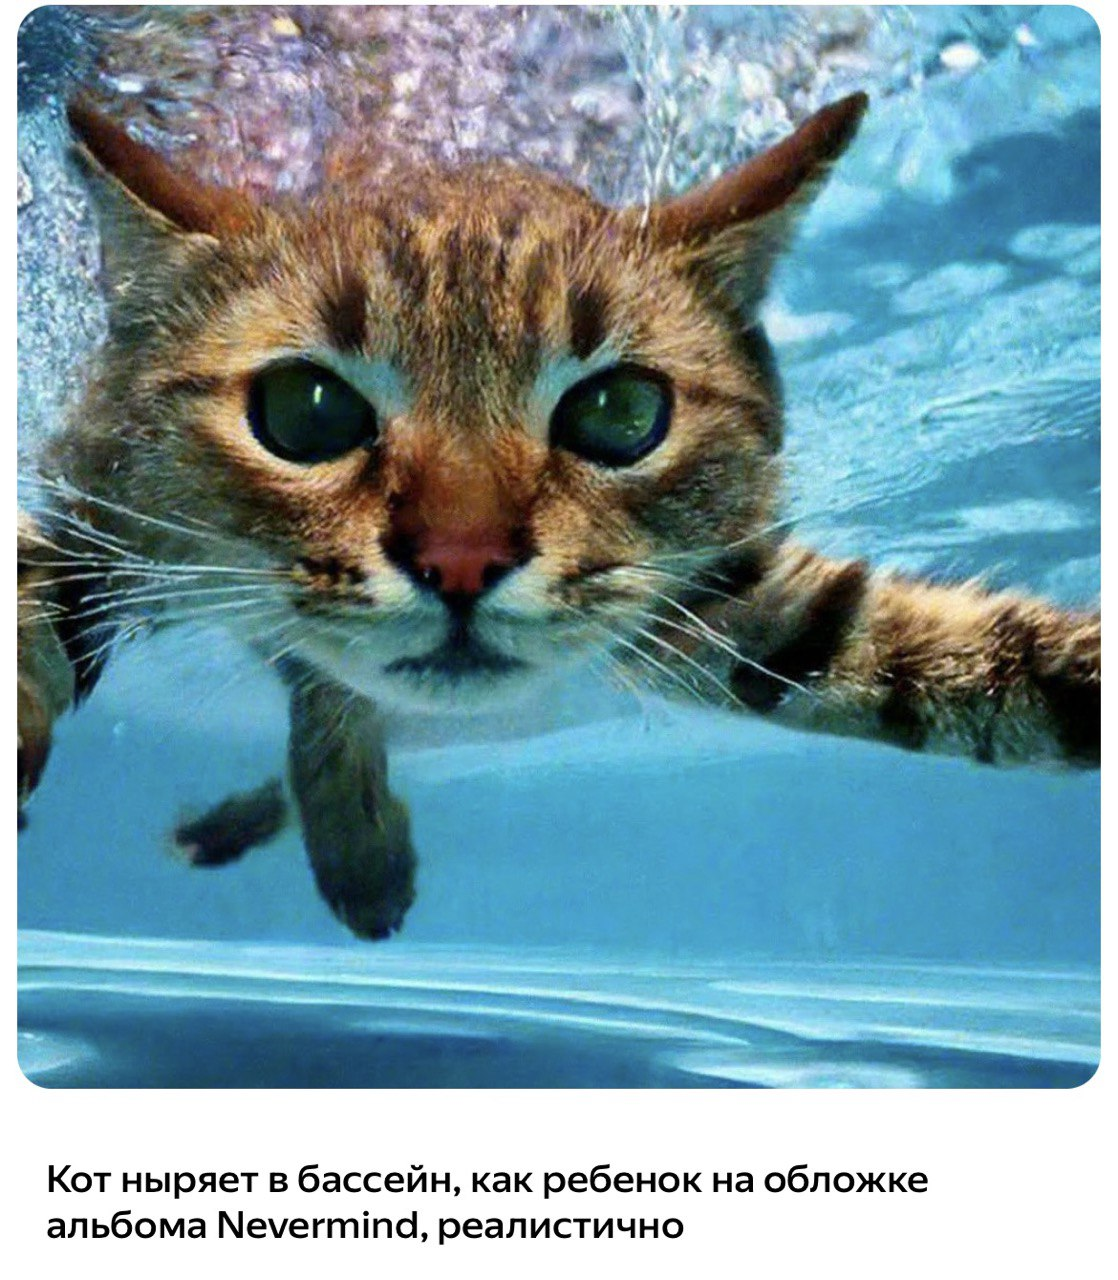
\includegraphics[width=0.9\linewidth]{figs/shedevrum1}
		\end{figure}
	\end{minipage}%
	\begin{minipage}[t]{0.5\columnwidth}
		\begin{figure}
			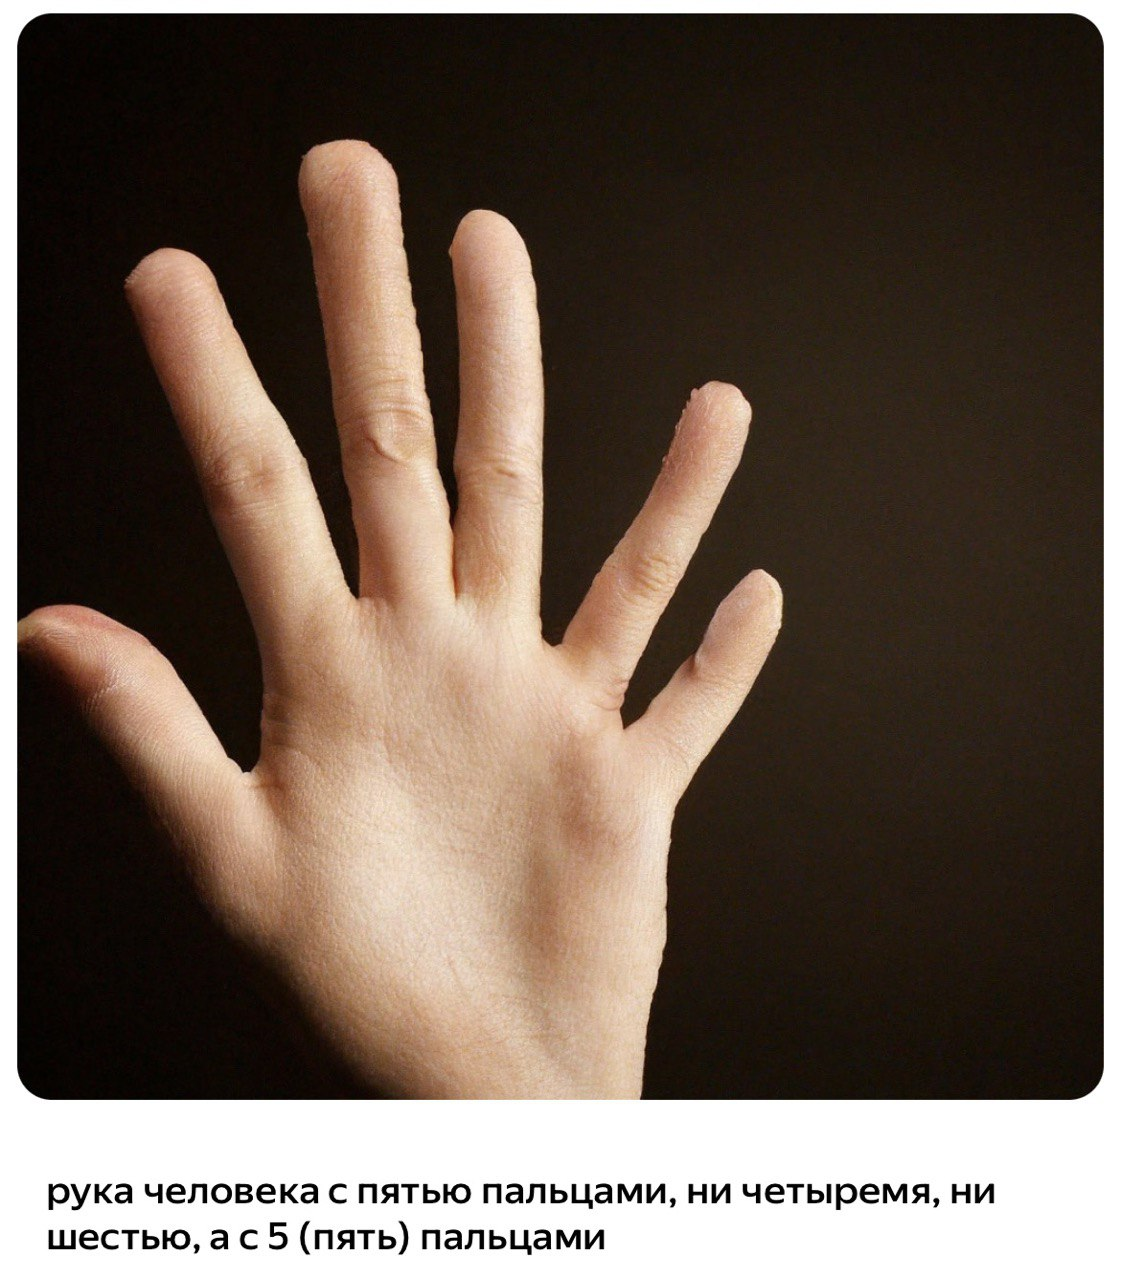
\includegraphics[width=0.9\linewidth]{figs/shedevrum2}
		\end{figure}
	\end{minipage}
\end{frame}
%=======
\begin{frame}{Conditional Models}
	In practice, we're typically interested in learning conditional models (sampling from conditional distribution~$\pd(\bx | \by)$). 
	\begin{itemize}
		\item $\by = \emptyset$, $\bx$ = image $\quad\Rightarrow\quad$ unconditional image model
		\item $\by$ = class label, $\bx$ = image $\quad\Rightarrow\quad$ class-conditional image model
		\item $\by$ = text prompt, $\bx$ = image $\quad\Rightarrow\quad$ text-to-image model
		\item $\by$ = image, $\bx$ = image $\quad\Rightarrow\quad$ image-to-image model
		\item $\by$ = image, $\bx$ = text $\quad\Rightarrow\quad$ image-to-text (image captioning) model
		\item $\by$ = English text, $\bx$ = Russian text $\quad\Rightarrow\quad$ sequence-to-sequence model (machine translation) model
		\item $\by$ = sound, $\bx$ = text $\quad\Rightarrow\quad$ speech-to-text (automatic speech recognition) model
		\item $\by$ = text, $\bx$ = sound $\quad\Rightarrow\quad$ text-to-speech model
	\end{itemize}
\end{frame}
%=======
\begin{frame}{Label Guidance}
	\myfootnotewithlink{https://arxiv.org/abs/1906.00446}{Razavi A., Oord A., et al. Generating Diverse High-Fidelity Images with VQ-VAE-2, 2019}
	\textbf{Label:} Ostrich (10th ImageNet class) 
	\begin{figure}
		\includegraphics[width=\linewidth]{figs/label_conditioning}
	\end{figure}
\end{frame}
%=======
\begin{frame}{Text Guidance}
	\myfootnotewithlink{https://arxiv.org/pdf/2112.10741}{Nichol A., et al. GLIDE: Towards Photorealistic Image Generation and Editing with Text-Guided Diffusion Models, 2022}
	\textbf{Prompt:} a stained glass window of a panda eating bamboo \\
	Left: $\gamma = 1$, Right: $\gamma = 3$.
	\begin{figure}
		\includegraphics[width=\linewidth]{figs/cfg}
	\end{figure}
\end{frame}
%=======
\begin{frame}{Guidance in Generative Models}
	\begin{block}{How to make guided model?}
		Instead of sampling from $\pt(\bx)$, we sample from $\pt(\bx | \by)$.
	\end{block}
	\eqpause
	Given \textbf{supervised} data $\{(\bx_i, \by_i)\}_{i=1}^n$, we can treat $\by$ as an additional model input:
	\eqpause
	\begin{itemize}
		\item $\pt(x_j | \bx_{1:j-1}, {\color{olive}\by})$ for AR models;
		\eqpause
		\item Encoder $q_{\bphi}(\bz | \bx, {\color{olive}\by})$ and decoder $\pt(\bx | \bz, {\color{olive}\by})$ for VAEs;
		\eqpause
		\item $G_{\btheta}(\bz, {\color{olive}\by})$ for NFs and GANs;
		\eqpause
		\item $\pt(\bx_{t-1} | \bx_t, {\color{olive}\by})$ for DDPMs.
	\end{itemize}
	\eqpause
	\begin{block}{Challenge}
		\begin{itemize}
			\item Empirically, images sampled with this procedure do not fit well enough to the desired label $\by$.
			\item Being able to control the strength of guidance is especially valuable.
		\end{itemize}
	\end{block}
\end{frame}
%=======
\subsection{Classifier Guidance}
%=======
\begin{frame}{Classifier Guidance}
	\myfootnotewithlink{https://arxiv.org/abs/2105.05233}{Dhariwal P., Nichol A. Diffusion Models Beat GANs on Image Synthesis, 2021}
	\begin{block}{DDPM Sampling}
		\begin{enumerate}
			\item Sample $\bx_T \sim \cN(0, \bI)$.
			\item Generate the denoised image (unconditional generation):
			\vspace{-0.3cm}
			\begin{align*}
				\bx_{t - 1} &= \frac{1}{\sqrt{1 - \beta_t}} \cdot \bx_t + \frac{\beta_t}{\sqrt{1 - \beta_t}} \cdot {\color{teal}\bs_{\btheta, t} (\bx_t)} +  \sigma_t \cdot \bepsilon \\
				\nextonslide{
				& = \frac{1}{\sqrt{1 - \beta_t}} \cdot \bx_t + \frac{\beta_t}{\sqrt{1 - \beta_t}} \cdot {\color{teal} \nabla_{\bx_t} \log \pt(\bx_t)} +  \sigma_t \cdot \bepsilon
				}
			\end{align*}
			\vspace{-0.5cm}
		\end{enumerate}
	\end{block}
	\eqpause
	\begin{block}{Guided Generation}
		\vspace{-0.5cm}
		\[
			\bx_{t - 1} = \frac{1}{\sqrt{1 - \beta_t}}\cdot \bx_t +  \frac{\beta_t}{\sqrt{1 - \beta_t}}  \cdot  \nabla_{\bx_t} \log \pt(\bx_t | {\color{olive}\by}) +  \sigma_t \cdot \bepsilon
		\]
		\vspace{-0.3cm}
	\end{block}
	\eqpause
	What is the link between $\nabla_{\bx_t} \log \pt(\bx_t)$ and $\nabla_{\bx_t} \log \pt(\bx_t | {\color{olive}\by})$?
\end{frame}
%=======
\begin{frame}{Classifier Guidance: Guided Score Function}
	\myfootnotewithlink{https://arxiv.org/abs/2105.05233}{Dhariwal P., Nichol A. Diffusion Models Beat GANs on Image Synthesis, 2021}
	\begin{block}{Guided Generation}
		\vspace{-0.5cm}
		\[
			\bx_{t - 1} = \frac{1}{\sqrt{1 - \beta_t}}\cdot \bx_t +  \frac{\beta_t}{\sqrt{1 - \beta_t}}  \cdot {\color{olive} \nabla_{\bx_t} \log \pt(\bx_t | \by)} +  \sigma_t \cdot \bepsilon
		\]
		\vspace{-0.5cm}
	\end{block}
	\eqpause
	\begin{block}{Guided Generation}
		\vspace{-0.7cm}
		\begin{align*}
			{\color{olive}\nabla_{\bx_t} \log \pt(\bx_t | \by)} &= \nabla_{\bx_t} \log \left(\frac{\pt(\bx_t)p(\by | \bx_t)}{p(\by)} \right)\\
			\nextonslide{
			&= {\color{violet}\nabla_{\bx_t} \log \pt(\bx_t)} + \nabla_{\bx_t} \log p(\by | \bx_t) \\
			}
			\nextonslide{
			&= {\color{violet} \bs_{\btheta, t}(\bx_t)} + {\color{teal}\nabla_{\bx_t} \log p(\by | \bx_t)}
			}
		\end{align*}
	\end{block}
	\vspace{-0.5cm}
	\eqpause
	\begin{block}{Guided Score Function}
		\vspace{-0.3cm}
		\[
			\bs_{\btheta, t}(\bx_t, \by) = \nabla_{\bx_t} \log \pt(\bx_t | \by).
		\]
		\eqpause
		\vspace{-0.3cm}
		\[
			{\color{olive}\bs_{\btheta, t}(\bx_t, \by)} = {\color{violet}\bs_{\btheta, t}(\bx_t)} + {\color{teal}\nabla_{\bx_t} \log p(\by | \bx_t)}
		\]
	\end{block}
\end{frame}
%=======
\begin{frame}{Classifier Guidance: Guidance Scale}
	\myfootnotewithlink{https://arxiv.org/abs/2105.05233}{Dhariwal P., Nichol A. Diffusion Models Beat GANs on Image Synthesis, 2021}
	\begin{block}{Guided Score Function}
		\vspace{-0.3cm}
		\[
			{\color{olive}\bs_{\btheta, t}(\bx_t, \by)} = \bs_{\btheta, t}(\bx_t) + \nabla_{\bx_t} \log p(\by | \bx_t)
		\]
		\vspace{-0.5cm}
	\end{block}
	\eqpause
	\begin{itemize}
		\item Let us assume $\by$ is a class label.
		\item $p(\by | \bx_t)$ is a classifier for noisy inputs.
		\item $p(\by | \bx_t)$ is responsible for model guidance.
	\end{itemize}
	\eqpause
	\begin{block}{Guidance Scale}
		It is a natural idea to scale up the contribution of the guidance
		\[
			{\color{violet}\bs^{\gamma}_{\btheta, t}(\bx_t, \by)} = \bs_{\btheta, t}(\bx_t) + {\color{teal}\gamma} \cdot \nabla_{\bx_t} \log p(\by | \bx_t)
		\]
		\eqpause
		\vspace{-0.5cm}
		\begin{itemize}
			\item The {\color{teal}guidance scale $\gamma$} adjusts the strength of classifier guidance.
			\item ${\color{violet}\bs^{\gamma}_{\btheta, t}(\bx_t, \by)}$ is not the true guided score function ${\color{olive}\bs_{\btheta, t}(\bx_t, \by)}$.
		\end{itemize}
	\end{block}
\end{frame}
%=======
\begin{frame}{Classifier Guidance: Distribution Sharpening}
	\myfootnotewithlink{https://arxiv.org/abs/2105.05233}{Dhariwal P., Nichol A. Diffusion Models Beat GANs on Image Synthesis, 2021}
	\begin{block}{Scaled Guided Score Function}
		\[
			{\color{violet}\bs^{\gamma}_{\btheta, t}(\bx_t, \by)} = \bs_{\btheta, t}(\bx_t)+ {\color{teal}\gamma} \cdot \nabla_{\bx_t} \log p(\by | \bx_t)
		\]
		\vspace{-0.5cm}
	\end{block}
	\eqpause
	\begin{block}{Scaled Conditional Distribution}
		\vspace{-0.5cm}
		\begin{align*}
			{\color{violet}\nabla_{\bx_t}^{\gamma} \log \pt(\bx_t | \by)} 
			&= \nabla_{\bx_t} \log \pt(\bx_t) + {\color{teal}\gamma}  \cdot \nabla_{\bx_t} \log p(\by | \bx_t) \\
			\nextonslide{
			&= \nabla_{\bx_t} \log \pt(\bx_t) + \nabla_{\bx_t} \log p(\by | \bx_t)^{\color{teal}\gamma} \\
			}
			\nextonslide{
			&= \nabla_{\bx_t} \log \left( \frac{\pt(\bx_t) p(\by | \bx_t)^{\gamma}}{Z} \right)
			}
		\end{align*}
		\vspace{-0.3cm}
	\end{block}
	\eqpause
	\textbf{Note:} Increasing $\gamma$ sharpens $p(\by | \bx_t)$, making it more contrast
	\[
		\hat{p}(\by | \bx_t) \propto p(\by | \bx_t)^{\gamma}.
	\]
\end{frame}
%=======
\begin{frame}{Classifier Guidance: Overview}
	\myfootnotewithlink{https://arxiv.org/abs/2105.05233}{Dhariwal P., Nichol A. Diffusion Models Beat GANs on Image Synthesis, 2021}

	\begin{block}{Training}
		\begin{itemize}
			\item Train the DDPM as before.
			\item Train an additional classifier $p(\by | \bx_t)$ on noisy data (note that it is dependent on time $t$).
		\end{itemize}
		\vspace{-0.2cm}
	\end{block}
	\eqpause
	\begin{block}{Guided DDPM Sampling}
		\begin{enumerate}
			\item Sample $\bx_T \sim \cN(0, \bI)$.
			\item Generate the denoised image (using scaled guided score function):
			\[
				\bx_{t-1} = \frac{1}{\sqrt{\alpha_t}} \cdot \bx_t + \frac{\beta_t}{\sqrt{1 - \beta_t}} \cdot  {\color{olive}\bs^{\gamma}_{\btheta, t}(\bx_t, \by)} + \sigma_t \cdot \bepsilon
			\]
		\end{enumerate}
	\end{block}
\end{frame}
%=======
\subsection{Classifier-Free Guidance}
%=======
\begin{frame}{Classifier-Free Guidance}
	\myfootnotewithlink{https://arxiv.org/abs/2207.12598}{Ho J., Salimans T. Classifier-Free Diffusion Guidance, 2022}
	\begin{itemize}
		\item The previous approach relies on training an additional classifier $p(\by | \bx_t)$ for noisy images.	
		\item We now introduce a method to sidestep this requirement.
	\end{itemize}
	\eqpause
	\[
		\nabla_{\bx_t}^{\gamma} \log \pt(\bx_t | \by) = \nabla_{\bx_t} \log \pt(\bx_t) + \gamma \cdot {\color{teal}\nabla_{\bx_t} \log p(\by | \bx_t)}
	\]
	\eqpause
	\vspace{-0.5cm}
	\begin{block}{Bayes theorem}
		\vspace{-0.7cm}
		\begin{align*}
			{\color{teal}\nabla_{\bx_t} \log p(\by | \bx_t)} &= \nabla_{\bx_t} \log \left( \frac{\pt(\bx_t| \by) p(\by)}{\pt(\bx_t)} \right) \\
			\nextonslide{
			&=  \nabla_{\bx_t} \log \pt(\bx_t| \by) -\nabla_{\bx_t} \log  \pt(\bx_t)
			}
		\end{align*}
	\end{block}
	\eqpause
	\vspace{-0.5cm}
	\begin{block}{Scaled Guided Score Function}
		\vspace{-0.7cm}
		\begin{multline*}
			\nabla_{\bx_t}^{\gamma} \log \pt(\bx_t | \by) = \nabla_{\bx_t} \log \pt(\bx_t) + \gamma \cdot {\color{teal} \nabla_{\bx_t} \log p(\by | \bx_t)}
			\nextonslide{ = \\ = \nabla_{\bx_t} \log \pt(\bx_t) + \gamma \cdot \bigl( {\color{teal}\nabla_{\bx_t} \log \pt(\bx_t| \by) - \nabla_{\bx_t} \log  \pt(\bx_t)} \bigr)}
			\nextonslide{ = \\ =  (1 - \gamma) \cdot  \nabla_{\bx_t} \log \pt(\bx_t) + \gamma \cdot  \nabla_{\bx_t} \log \pt(\bx_t| \by)}
		\end{multline*}
	\end{block}
\end{frame}
%=======
\begin{frame}{Classifier-Free Guidance: Formulation}
	\myfootnotewithlink{https://arxiv.org/abs/2207.12598}{Ho J., Salimans T. Classifier-Free Diffusion Guidance, 2022}
	\begin{block}{Scaled Guided Score Function}
		\vspace{-0.5cm}
		\[
			\nabla_{\bx_t}^{\gamma} \log \pt(\bx_t | \by) =  (1 - \gamma) \cdot  \nabla_{\bx_t} \log \pt(\bx_t) + \gamma \cdot  \nabla_{\bx_t} \log \pt(\bx_t| \by)
		\]
		\vspace{-0.5cm}
		\eqpause
		\[
			\bs^{\gamma}_{\btheta, t}(\bx_t, \by) = (1 - \gamma) \cdot \bs_{\btheta, t}(\bx_t) +  \gamma \cdot \bs_{\btheta, t}(\bx_t, \by)
		\]
		\vspace{-0.5cm}
	\end{block}
	\eqpause
	\begin{block}{Naive training approach}
		\begin{itemize}
			\item Train an unguided score function model $\bs_{\btheta, t}(\bx_t)$.
			\item Train a guided score function model $\bs_{\btheta, t}(\bx_t, \by)$.
			\eqpause
			\item Use their convex combination at inference.
		\end{itemize}
	\end{block}
	\begin{block}{Guided Sampling}
		\vspace{-0.3cm}
		\[
			\bx_{t-1} = \frac{1}{\sqrt{\alpha_t}} \cdot \bx_t + \frac{\beta_t}{\sqrt{1 - \beta_t}} \cdot  {\color{olive}\bs^{\gamma}_{\btheta, t}(\bx_t, \by)} + \sigma_t \cdot \bepsilon
		\]
		\vspace{-0.3cm}
	\end{block}
	\eqpause
	How to avoid training two separate score function models?
\end{frame}
%=======
\begin{frame}{Classifier-Free Guidance}
	\myfootnotewithlink{https://arxiv.org/abs/2506.02070}{Holderrieth P., Erives E. An Introduction to Flow Matching and Diffusion Models, 2025}
	\[
		\bs^{\gamma}_{\btheta, t}(\bx_t, \by) = (1 - \gamma) \cdot \bs_{\btheta, t}(\bx_t) +  \gamma \cdot \bs_{\btheta, t}(\bx_t, \by)
	\]
	\vspace{-0.5cm}
	\begin{block}{CFG algorithm}
		\begin{itemize}
			\item Introduce "the absence of conditioning" label $\by = \varnothing$.		
			\eqpause
			\item Use it to get unguided score function $\bs_{\btheta, t}(\bx_t) = \bs_{\btheta, t}(\bx_t, \varnothing)$.		
			\eqpause
			\item Train a single model $\bs_{\btheta, t}(\bx_t, \by)$ using \textbf{supervised} data, but artificially drop the labels $\by$ with some fixed probability (simulating the case of $\by = \varnothing$).		
			\eqpause
			\item Apply the model twice during inference to get $\bs_{\btheta, t}(\bx_t, \varnothing)$ and $\bs_{\btheta, t}(\bx_t, \by)$.
		\end{itemize}
	\end{block}
	\vspace{-0.3cm}
	\eqpause
	\begin{block}{Guided Sampling}
		\vspace{-0.3cm}
		\[
			\bx_{t-1} = \frac{1}{\sqrt{\alpha_t}} \cdot \bx_t + \frac{\beta_t}{\sqrt{1 - \beta_t}} \cdot  {\color{olive}\bs^{\gamma}_{\btheta, t}(\bx_t, \by)} + \sigma_t \cdot \bepsilon
		\]
		\vspace{-0.3cm}
	\end{block}
\end{frame}
%=======
\section{Continuous-Time Normalizing Flows}
%=======
\begin{frame}{Discrete-Time Normalizing Flows}
	\myfootnotewithlink{https://lilianweng.github.io/lil-log/2018/10/13/flow-based-deep-generative-models.html}{https://lilianweng.github.io/lil-log/2018/10/13/flow-based-deep-generative-models.html}
	\vspace{-0.3cm}
	\begin{block}{Change of Variable Theorem (CoV)}
		Let $\bx$ be a random variable with density $p(\bx)$, and let $\bff: \bbR^m \rightarrow \bbR^m$ be a differentiable and \textbf{invertible} transformation. If $\bz = \bff(\bx)$, $\bx = \bff^{-1}(\bz) = \bg(\bz)$, then
		\vspace{-0.3cm}
		\[
			p(\bx) = p(\bz) |\det(\bJ_{\bff})| = p(\bz) \left|\det \left( \frac{\partial \bz}{\partial \bx} \right) \right| = p(\bff(\bx)) \left|\det \left(  \frac{\partial \bff(\bx)}{\partial \bx} \right) \right|
		\]
		\vspace{-0.5cm}
	\end{block}
	\eqpause

	\vspace{-0.3cm}
	\begin{figure}
		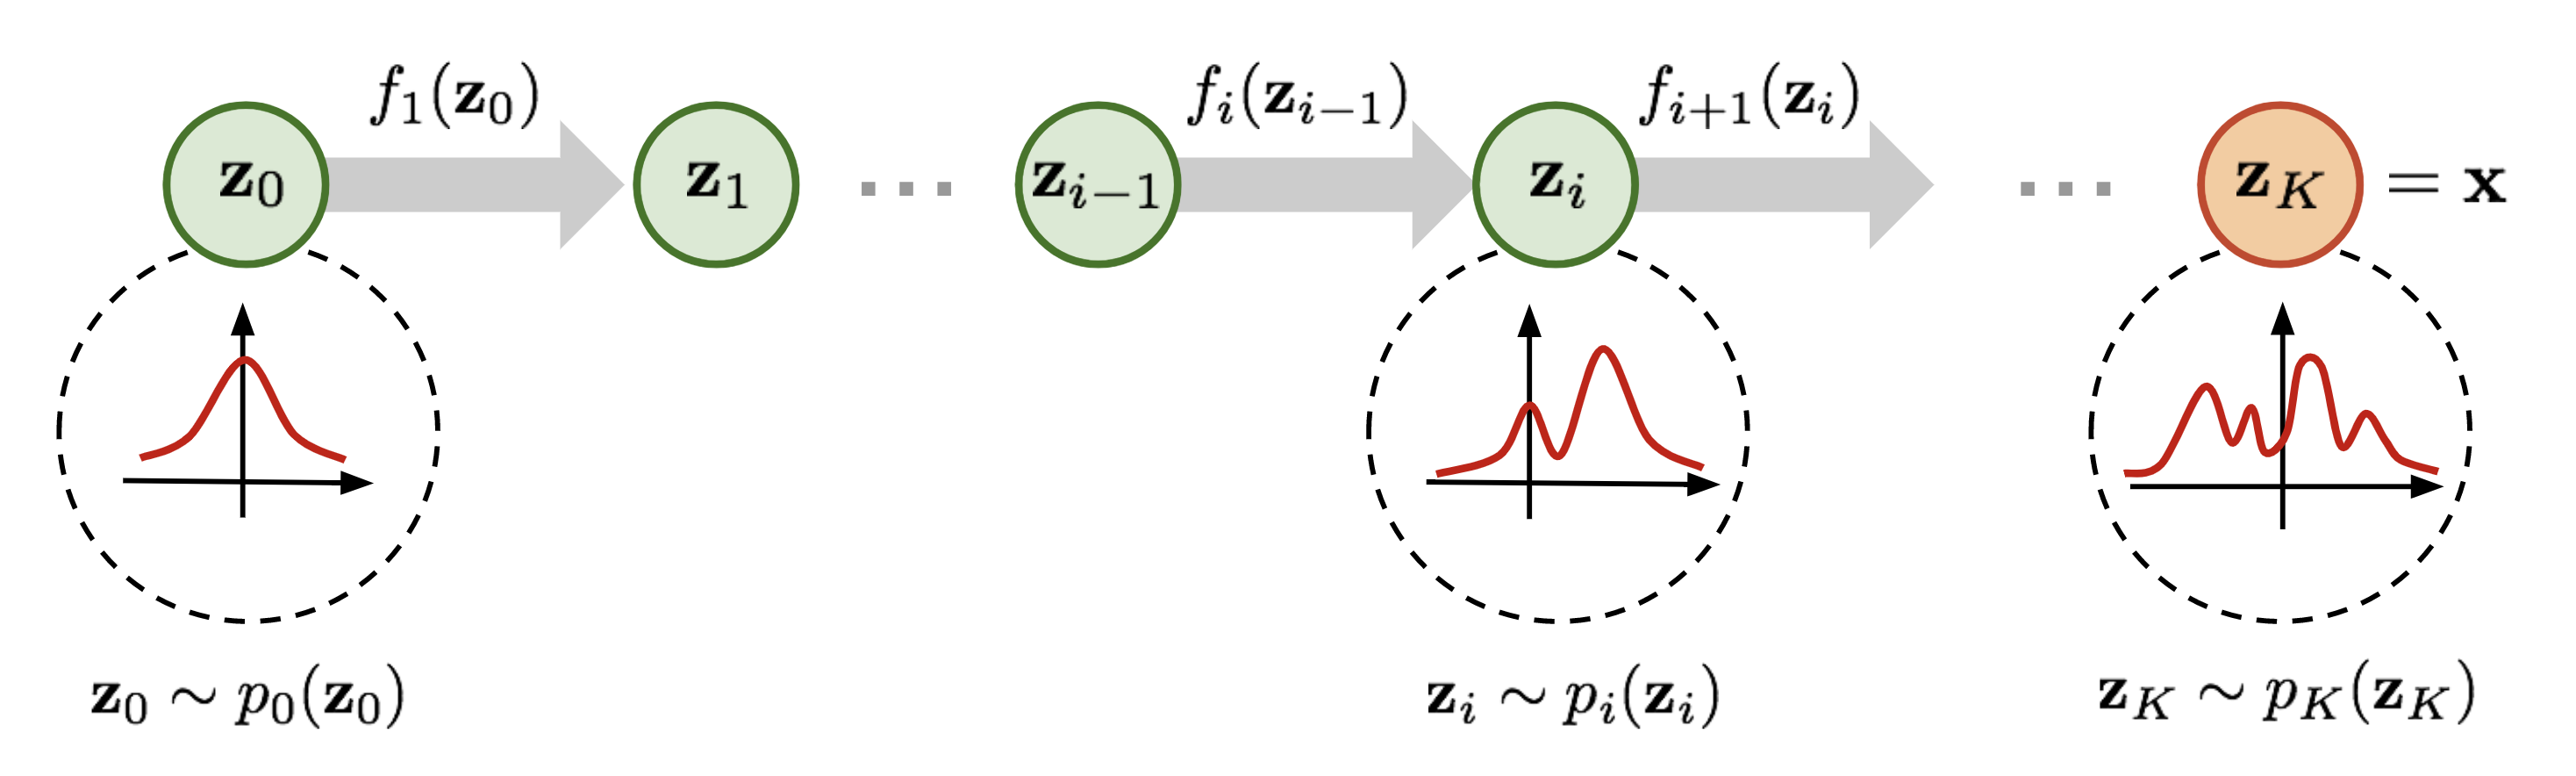
\includegraphics[width=0.95\linewidth]{figs/normalizing-flow}
	\end{figure}
	\vspace{-0.4cm}
	\[
		\log \pt(\bx) = \log p(\bff_K \circ \dots \circ \bff_1(\bx)) + \sum_{k=1}^K\log \left|\det \left(\frac{\partial \bff_k}{\partial \bff_{k-1}}\right)\right|.
	\]
	\vspace{-0.4cm}
\end{frame}
%=======
\begin{frame}{Towards Continuous-Time Normalizing Flows}
	\begin{itemize}
		\item Up to this point, we have considered discrete-time normalizing flows:
		\vspace{-0.3cm}
		 \[
		 	 \bx_{t+1} = \bff_{\btheta}(\bx_t, t); \quad \log p(\bx_{t+1}) = \log p(\bx_{t}) - \log \left| \det \frac{\partial \bff_{\btheta}(\bx_t)}{\partial \bx_{t}} \right| .
		 \]
		\item Let us now move to the general case of continuous time, using a mapping $\bx(t): \bbR \rightarrow \bbR^m$ to describe continuous dynamics.
	\end{itemize}
	\eqpause
	\begin{block}{Continuous-Time Dynamics}
		Consider an Ordinary Differential Equation (ODE):
		\vspace{-0.3cm}
		\begin{align*}
		   \frac{d \bx(t)}{dt} &= \bff_{\btheta}(\bx(t), t); \quad \text{with initial condition }\bx(t_0) = \bx_0. \\
		   \nextonslide{
		   \bx(t_1) &= \int^{t_1}_{t_0} \bff_{\btheta}(\bx(t), t) d t  + \bx_0
		   }
		\end{align*}
		\vspace{-0.6cm}
	\end{block}
	Here, $\bff_{\btheta}: \bbR^m \times [t_0, t_1] \rightarrow \bbR^m$ is a \textbf{vector field}.
\end{frame}
%=======
\begin{frame}{Ordinary Differential Equations (ODEs)}
	\begin{align*}
		\frac{d \bx(t)}{dt} &= \bff_{\btheta}(\bx(t), t); \quad \text{with initial condition }\bx(t_0) = \bx_0. \\
		\bx(t_1) &= \int^{t_1}_{t_0} \bff_{\btheta}(\bx(t), t) d t  + \bx_0
	\end{align*}
	\vspace{-0.6cm}
	\begin{block}{Flow}
		Let call \textbf{the flow} $\bpsi: \bbR^m \times [t_0, t_1] \rightarrow \bbR^m$ the solution of ODE:
		\[
			\frac{d \bpsi_t(\bx_0)}{dt} = \bff_{\btheta}(\bpsi_t(\bx_0), t); \quad \text{with initial condition }\bpsi_0(\bx_0) = \bx_0.
		\]
	\end{block}
	\begin{block}{Numerical Solution of ODEs}
		\vspace{-0.5cm}
		\[
			\bpsi_t(\bx_0) = \int^{t_1}_{t_0} \bff_{\btheta}(\bx(t), t) d t  + \bx_0 \nextonslide{\approx {\color{teal}\texttt{ODESolve}_f(\bx_0, \btheta, t_0, t_1)}.}
		\]
		\eqpause
		Here, we require the numerical routine $\texttt{ODESolve}_f(\bx_0, \btheta, t_0, t_1)$.
	\end{block}
\end{frame}
%=======
\begin{frame}{Numerical Solution of ODEs}
	\myfootnotewithlink{https://en.wikipedia.org/wiki/Heun's\_method}{Image credit: https://en.wikipedia.org/wiki/Heun's\_method}   
	\[
		\bpsi_t(\bx_0) = \int^{t_1}_{t_0} \bff_{\btheta}(\bx(t), t) d t  + \bx_0 \approx {\color{teal}\texttt{ODESolve}_f(\bx_0, \btheta, t_0, t_1)}.
	\]
	$\texttt{ODESolve}_f(\bx_0, \btheta, t_0, t_1)$ consists of sequence of iterative update steps.
	\eqpause
	\begin{block}{Euler Update Step}
		\begin{minipage}[t]{0.5\columnwidth}
			\vspace{-0.3cm}
			\[
	  			\frac{\bx(t + h) - \bx(t)}{h} = \bff_{\btheta}(\bx(t), t)
			\]
			\[
	  			\bx(t + h) = \bx(t) + h \cdot \bff_{\btheta}(\bx(t), t)
			\]
		\end{minipage}%
		\eqpause
		\begin{minipage}[t]{0.5\columnwidth}
			\vspace{-0.8cm}
			\begin{figure}
				\centering
				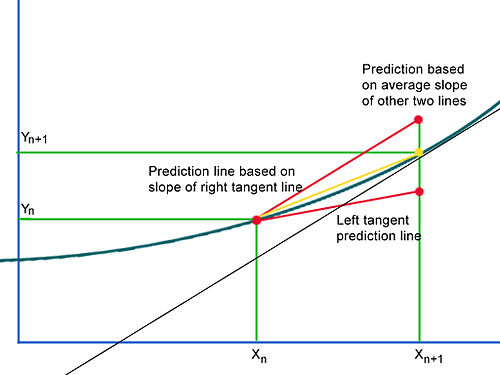
\includegraphics[width=\linewidth]{figs/heun_method}
			\end{figure}
		\end{minipage}
	\end{block}
	\vspace{-1.0cm}
	\begin{block}{Heun's Update Step}
		\vspace{-0.3cm}
		\[
			\bx'(t + h) = \bx(t) + h \cdot \bff_{\btheta}(\bx(t), t)
		\]
		\[
			\bx(t + h) = \bx(t) + \frac{h}{2} \cdot \left(\bff_{\btheta}(\bx(t), t) + \bff_{\btheta}(\bx'(t+h), t + h)\right)
		\]
	\end{block}
\end{frame}
%=======
\begin{frame}{Continuous-Time Normalizing Flows: Neural ODE}
	\myfootnotewithlink{https://arxiv.org/abs/1806.07366}{Chen R. T. Q. et al. Neural Ordinary Differential Equations, 2018}   
	\begin{block}{Neural ODE}
		\vspace{-0.2cm}
		\[
  			\frac{d \bx(t)}{dt} = \bff_{\btheta}(\bx(t), t); \quad \text{with initial condition }\bx(t_0) = \bx_0
		\]
		\vspace{-0.3cm}
	\end{block}
	\begin{block}{Euler \texttt{ODESolve}}
		\vspace{-0.3cm}
		\[
		    \bx(t + h) = \bx(t) + h \cdot \bff_{\btheta}(\bx(t), t)
		\]
		\vspace{-0.5cm}
	\end{block}
	\eqpause
	\begin{itemize}
		\item Consider $[t_0, t_1] = [0, 1]$ for simplicity.
		\item If $\bx(0)$ is a random variable with density~$p_0(\bx)$,
		\item Then, for any $t$, $\bx(t)$ is a random variable with density $p_t(\bx)$.
	\end{itemize}
\end{frame}
%=======
\begin{frame}{Continuous-Time Normalizing Flows: Intuition}
	\myfootnotewithlink{https://arxiv.org/abs/1810.01367}{Grathwohl W. et al. FFJORD: Free-form Continuous Dynamics for Scalable Reversible Generative Models, 2018}  
	\[
 		\frac{d \bx(t)}{dt} = \bff_{\btheta}(\bx(t), t); \quad \text{with initial condition }\bx(t_0) = \bx_0
	\]
	\eqpause
	\vspace{-0.5cm}
	\begin{itemize}
		\item $p_t(\bx) = p(\bx, t)$ describes the \textbf{probability path} interpolating between $p_0(\bx)$ and $p_1(\bx)$.
		\item {\color{gray}What is the difference between $p_t(\bx(t))$ and $p_t(\bx)$?}
	\end{itemize}
	\eqpause
	\begin{figure}
		\centering
		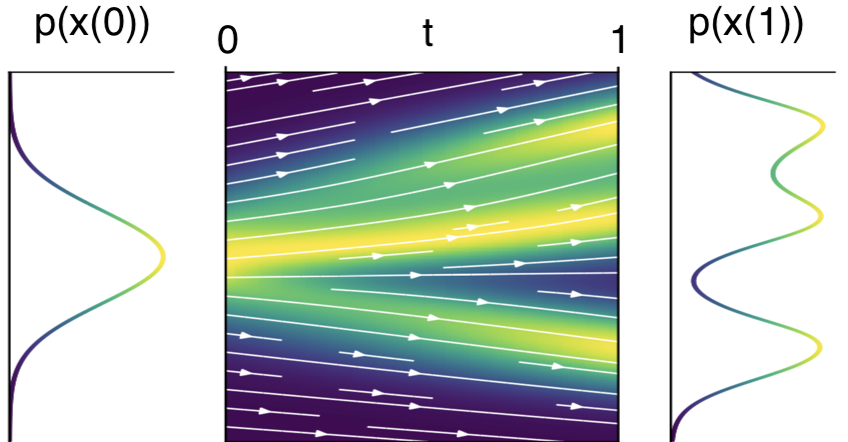
\includegraphics[width=0.75\linewidth]{figs/cnf_flow.png}
	\end{figure}
\end{frame}
%=======
\begin{frame}{Continuous-Time Normalizing Flows: Reversibility}
	\myfootnotewithlink{https://arxiv.org/abs/1806.07366}{Chen R. T. Q. et al. Neural Ordinary Differential Equations, 2018}   
	\begin{block}{Theorem (Picard)}
		If $\bff$ is continuously differentiable with a bounded derivative in $\bx$ and continuous in $t$, then the ODE has a \textbf{unique solution} given by a flow $\bpsi_t$.
	\end{block}
	\eqpause
	This guarantees the ODE is \textbf{uniquely reversible}. 
	\begin{align*}
		\bpsi_1(\bx_0) &= \bx_0 + \int_{0}^{1} \bff_{\btheta}(\bpsi_t(\bx_0), t) dt \\
		\bx(1) &= \bx(0) + \int_{0}^{1} \bff_{\btheta}(\bx(t), t) dt \\
		\bx(0) &= \bx(1) + \int_{1}^{0} \bff_{\btheta}(\bx(t), t) dt
	\end{align*}
	\eqpause
	\textbf{Note:} Unlike discrete-time flows, $\bff$ need not be invertible (uniqueness ensures bijection).
	\eqpause
	How can we compute $p_t(\bx)$ at arbitrary $t$?
\end{frame}
%=======
\begin{frame}{Summary}
	\begin{itemize}
		\item DDPM and NCSN are intimately connected at the objective level.	
		\vfill
		\item Classifier guidance provides a technique to turn an unconditional model into a conditional one by training an auxiliary classifier on noisy data.
		\vfill
		\item Classifier-free guidance removes the need for such a classifier, yielding a practical recipe now widely used.
		\vfill 
		\item Continuous-time normalizing flows leverage neural ODEs to define continuous-time trajectories $\bx(t)$, relaxing many constraints of discrete-time flows.
		\vfill
		\item If $\bx_0$ is a random variable, this yields a \textbf{probability path} $p_t(\bx)$ as time evolves.
	\end{itemize}
\end{frame}
%=======
\end{document}